%%%%%%%%%%%%%%%%%%%%%%%%%%%%%%%%%%%%%%%%%%%%%%%%%%%%%%%%%%%%%%%
%
% Welcome to Overleaf --- just edit your LaTeX on the left,
% and we'll compile it for you on the right. If you give 
% someone the link to this page, they can edit at the same
% time. See the help menu above for more info. Enjoy!
%
%%%%%%%%%%%%%%%%%%%%%%%%%%%%%%%%%%%%%%%%%%%%%%%%%%%%%%%%%%%%%%%

%  My thanks to Dana Ernst of Northern Arizona University for sharing 
%    his template with me. This is largely his work.
% --------------------------------------------------------------
% This is all preamble stuff that you don't have to worry about.
% Head down to where it says "Start here"
% --------------------------------------------------------------
 
\documentclass[12pt]{article}
 
\usepackage[margin=1in]{geometry} 
\usepackage{amsmath,amsthm,amssymb}
\usepackage{graphicx}
\usepackage{float}
\usepackage[table,x11names]{xcolor}
\usepackage[lined, linesnumbered]{algorithm2e}
\usepackage{tikz}
\makeatletter
\newenvironment{btHighlight}[1][]
{\begingroup\tikzset{bt@Highlight@par/.style={#1}}\begin{lrbox}{\@tempboxa}}
{\end{lrbox}\bt@HL@box[bt@Highlight@par]{\@tempboxa}\endgroup}

\newcommand\btHL[1][]{%
  \begin{btHighlight}[#1]\bgroup\aftergroup\bt@HL@endenv%
}
\def\bt@HL@endenv{%
  \end{btHighlight}%   
  \egroup
}
\newcommand{\bt@HL@box}[2][]{%
  \tikz[#1]{%
    \pgfpathrectangle{\pgfpoint{1pt}{0pt}}{\pgfpoint{\wd #2}{\ht #2}}%
    \pgfusepath{use as bounding box}%
    \node[anchor=base west, fill=orange!30,outer sep=0pt,inner xsep=1pt, inner ysep=0pt, rounded corners=3pt, minimum height=\ht\strutbox+1pt,#1]{\raisebox{1pt}{\strut}\strut\usebox{#2}};
  }%
}
\makeatother

\usepackage[listings,skins]{tcolorbox}
\tcbset{colback=gray!1!white,colframe=black}




\newenvironment{theorem}[2][Theorem]{\begin{trivlist}
\item[\hskip \labelsep {\bfseries #1}\hskip \labelsep {\bfseries #2.}]}{\end{trivlist}}
\newenvironment{lemma}[2][Lemma]{\begin{trivlist}
\item[\hskip \labelsep {\bfseries #1}\hskip \labelsep {\bfseries #2.}]}{\end{trivlist}}
\newenvironment{conjecture}[2][Conjecture]{\begin{trivlist}
\item[\hskip \labelsep {\bfseries #1}\hskip \labelsep {\bfseries #2.}]}{\end{trivlist}}
\newenvironment{question}[2][Question]{\begin{trivlist}
\item[\hskip \labelsep {\bfseries #1}\hskip \labelsep {\bfseries #2.}]}{\end{trivlist}}
\newenvironment{corollary}[2][Corollary]{\begin{trivlist}
\item[\hskip \labelsep {\bfseries #1}\hskip \labelsep {\bfseries #2.}]}{\end{trivlist}}
\newenvironment{definition}[2][Definition]{\begin{trivlist}
\item[\hskip \labelsep {\bfseries #1}\hskip \labelsep {\bfseries #2.}]}{\end{trivlist}}


\definecolor{commentgreen}{RGB}{176, 176, 176}
\definecolor{rowcolor}{cmyk}{0,0.87,0.68,0.32}
\definecolor{rowcolor2}{cmyk}{ 20, 0, 37, 34}

\definecolor{eminence}{RGB}{108,48,130}
\definecolor{weborange}{RGB}{255,165,0}
\definecolor{frenchplum}{RGB}{129,20,82}
\definecolor{darkgreen}{RGB}{10, 92, 10}


\definecolor{celadon}{rgb}{0.67, 0.88, 0.69}

\definecolor{mGreen}{rgb}{0,0.6,0}
\definecolor{mGray}{rgb}{0.5,0.5,0.5}
\definecolor{mPurple}{rgb}{0.58,0,0.82}
\definecolor{backgroundColour}{rgb}{0.95,0.95,0.92}

\lstdefinestyle{CStyle}{
    commentstyle=\color{mGreen},
    keywordstyle=\color{magenta},
    numberstyle=\tiny\color{mGray},
    stringstyle=\color{mPurple},
    basicstyle=\footnotesize,
    breakatwhitespace=false,         
    breaklines=true,                 
    captionpos=b,                    
    keepspaces=true,                 
    numbers=left,                    
    numbersep=5pt,                  
    showspaces=false,                
    showstringspaces=false,
    showtabs=false,                  
    tabsize=2,
    language=C,
    moredelim=**[is][{\btHL[celadon!40]}]{`}{`}
}

\lstdefinestyle{nccode}{
    numbers=none,
    stepnumber=1,
    numbersep=10pt,
    tabsize=4,
    showspaces=false,
    breaklines=true, 
    showstringspaces=false,
    moredelim=**[is][{\btHL[orange!50]}]{`}{`}
}

\begin{document}
 
% --------------------------------------------------------------
%                         Start here
% --------------------------------------------------------------
 
\title{Assignment 2: Programming with OpenMP} % replace with an appropriate title, choose something shortish & descriptive
\author{Javier Cabrera Arteaga} % replace with your name, multiple authors go in alphabetical order by last name
 
\maketitle

{%
\centering
FDD3258 - Introduction to High-Performance Computing
\par
}
\hrule
\vspace{.2in}


\section{Exercise 1 - OpenMP Hello World, get familiar with OpenMP Environment}


\begin{enumerate}
	\item Write an OpenMP C code with each thread printing Hello World from Thread X! where X is the thread ID.
	\begin{lstlisting}[style=CStyle]
#include <stdio.h>

int th_id, nthreads;

int main(void){

	#ifdef NUM_THREADS
		omp_set_num_threads(NUM_THREADS);
	#endif

	#pragma omp parallel private(th_id)
	{
		nthreads = omp_get_num_threads();
		th_id = omp_get_thread_num();
		printf("Hello, world %d/%d. \n", th_id, nthreads);
	}

	return 0;
}
	\end{lstlisting}
	\item Answers
	\begin{enumerate}
		\item To enable openmp in my local machine: \texttt{gcc-9 -fopenmp}.
		\item Ways to set the number of threads:
		\begin{enumerate}
			\item Before compiling, set the environment variable, \texttt{export OMP\_NUM\_THREADS=<num\_threads>}
			\item At runtime \texttt{omp\_set\_num\_threads()}
		\end{enumerate}
	\end{enumerate}
	
  
\end{enumerate}

\section{Exercise 2. STREAM benchmark and the importance of threads}

	\begin{enumerate}
		\item \textit{Prepare a plot (with Excel, Matlab, Gnuplot, …) comparing the bandwidth using 1-2-4-8-12-16-20-24-28-32 threads.}
		
		\begin{figure}[H]
			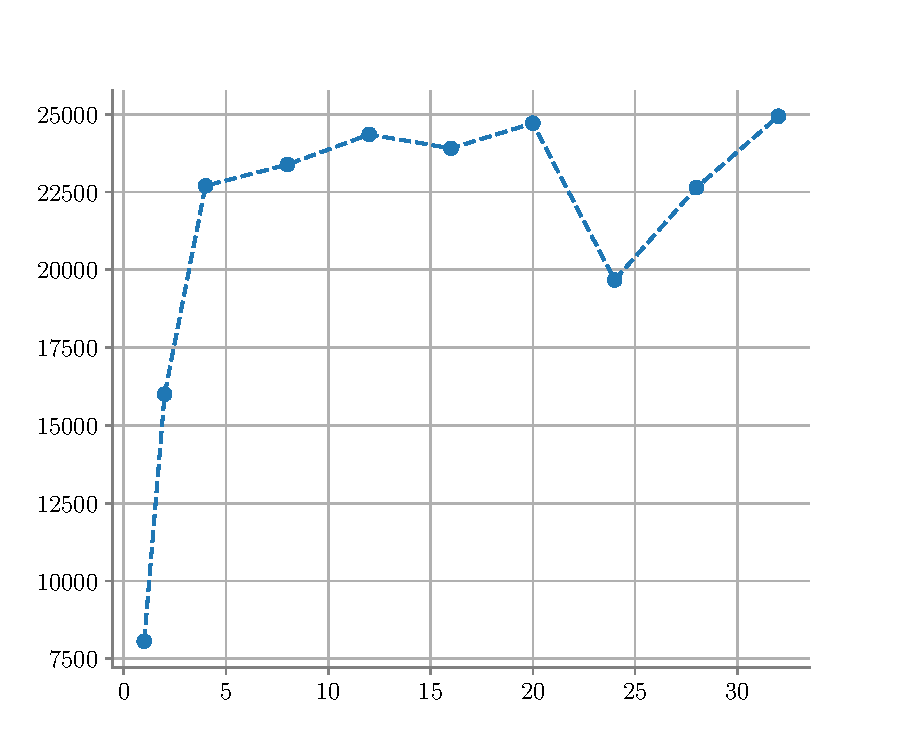
\includegraphics[width=0.8\textwidth]{stream.pdf}
		\end{figure}
		\item \textit{How does the bandwidth measured with copy kernel depend on the number of threads?}
		\item \textit{Prepare a plot comparing the bandwidth measured with copy kernel with static, dynamic and guided schedules using 32 threads.}
		\begin{figure}[H]
			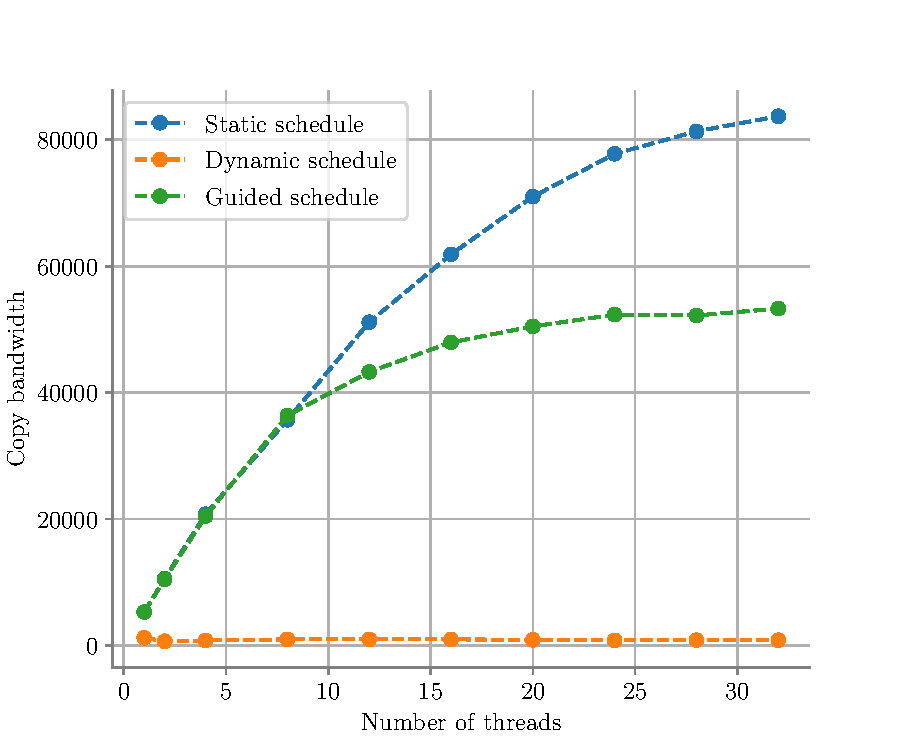
\includegraphics[width=0.8\textwidth]{stream2.pdf}
		\end{figure}
		\begin{enumerate}
			\item \textit{How do you set the schedule in the STREAM code? What is the fastest schedule and why do you think it is so?}
		\end{enumerate}

		
	\end{enumerate}
\end{document}